\chapter{Results}\label{ch:results}
This chapter covers the most important experiments and results that we have obtained. Additionally, we provide insights on how we proceeded, on technical aspects, and also some thought processes that influenced our decisions. Subsequently, we present our results for ansatzes and optimizers.

Before proceeding further, it is essential to clarify the following terms that will frequently appear in this chapter.

An \textit{iteration} is a single run of the VQE encompassing both quantum and classical parts. The number of iterations determines how many times ansatz will obtain a new set of optimized parameters.

When an optimization algorithm attempts to find the best parameters for an ansatz, it evaluates a cost function. \textit{Cost function evaluations} counts how many times the cost function was evaluated.

\section{Benchmark setup}
Our objective was to find the ground state energy of a hydrogen molecule and figure out some optimizations concerning ansatzes and optimizers. Initially, we started by trying to run the VQE with few different optimizers and ansatzes. Even though the ground state is just a real number, we wanted to know how the energy convergence progresses. We did that by plotting an energy convergence graph similar to that in Figure~\ref{fig:energy-convergence}. For illustration purposes, we chose two optimizers, \textit{COBYLA} and \textit{Gradient Descent}, and six ansatzes we mentioned in section~\ref{sec:ansatzes}.
\begin{figure}[H]
    \centering
    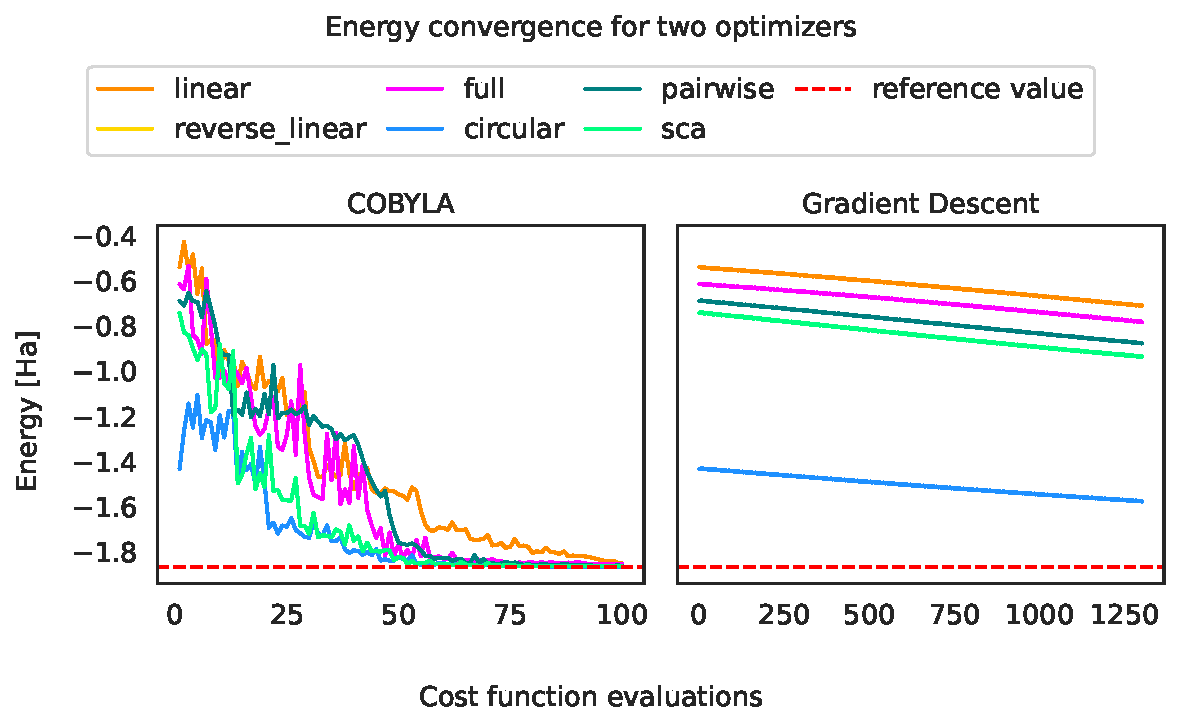
\includegraphics[width=\textwidth]{convergence_example.pdf}
    \caption{Examples of energy convergence for various optimizers}
    \label{fig:energy-convergence}
\end{figure}
From the above figure, we can observe that not only convergence to ground state energy but also cost function evaluations differ a lot. Some optimizers have a fixed number of cost function evaluations for each iteration, an amount of cost function evaluations in a single iteration depends on an optimizer's strategy. Another thing worth pointing out is that we benchmarked six ansatzes, however, we can see only five of them. The reverse linear ansatz is overlapped by the full ansatz since a matrix representation of the reverse linear ansatz is the same as the full ansatz. Observation of such big differences between multiple optimizers and ansatzes led us to the idea of benchmarking multiple ansatzes and optimizers and doing a further analysis of that. In the following subsections, we describe details of our benchmarking.

\subsection*{Ansatzes}
In our benchmark, we categorized ansatzes based on entanglement. We decided to go with 6 ansatzes, namely linear, reverse linear, full, circular, pairwise, and SCA as mentioned in section~\ref{sec:ansatzes}. From each ansatz, we created 3 variations, 1-layer, 2-layer, and 3-layer ansatzes. In total, we have 18 parametrized quantum circuits that we tried to run the VQE algorithm with.

\subsection*{Hamiltonian}
For all the experiments we used a 4-qubit Hamiltonian of a hydrogen molecule. We took it from a paper produced by Miháliková et al.~\cite{mihalikova} and it is defined as follows:

\begin{align*}H_{H_2}^{4-qubit} &= c_{0}1 + c_{1}Z_{0} + c_{2}Z_{1}Z_{0} + c_{1}Z_{2} + c_{2}Z_{3}Z_{2}Z_{1} + c_{3}Z_{1} + c_{4}Z_{2}Z_{0}\\
                                &+ c_{5}X_{2}Z_{1}X_{0} + c_{6}Z_{3}X_{2}X_{0} + c_{6}X_{2}X_{0} + c_{5}Z_{3}X_{2}Z_{1}X_{0}\\
                                &+c_{7}Z_{3}Z_{2}Z_{1}Z_{0} + c_{7}Z_{2}Z_{1}Z_{0} + c_{8}Z_{3}Z_{2}Z_{0} + c_{3}Z_{3}Z_{1}\text{,}
\end{align*}
where coefficients are:
\begin{alignat*}{3}
    &c_0 = -0.80718,\qquad &c_1 = 0.17374,\qquad &c_2 =-0.23047, \\
    &c_3 = 0.12149,\qquad  &c_4 = 0.16940,\qquad &c_5 = -0.04509, \\
    &c_6 = 0.04509,\qquad  &c_7 = 0.16658,\qquad &c_8 = 0.17511.
\end{alignat*}

This Hamiltonian can be further simplified to 2 qubits, however, we retained this form to increase the complexity of the problem. The ground state of this Hamiltonian is $-1.8671050114542505$, we calculated that using a \textit{NumPyMinimumEigensolver} algorithm provided by Qiskit and we will use this value as a reference value for our experiments. Plotting energy convergence graphs for multiple optimizers and ansatzes does not show well the proximity of the resulting energy to the ground state energy. Additionally, interpreting such a vast amount of data is challenging, making it difficult to draw conclusions or present findings effectively on paper. Hence, we will consider the probability of reaching a chemical precision. Chemical precision refers to how closely individual measurements agree with the correct value~\cite{chemistry}. The standard chemical precision is $0.0016$ Ha, a familiar value among chemists.

\subsection*{Optimizers}
After browsing some scientific articles we did not find any definite answer to which optimizers work the best. This was also one of the reasons why we decided to test almost all optimizers that Qiskit offers. Furthermore, optimizers have a plethora of parameters and configuring them would be a nightmare so we went with the default ones, except for the number of iterations. We set the number of iterations to 100 for each optimizer. Below are concise descriptions of all the tested optimizers, along with a summary table categorizing them by type.\\\\\\\\\\\\
\textbf{AQGD (Analytical Quantum Gradient Descent)}~\cite{aqgd}:
\begin{itemize}
    \item The algorithm proposed specifically for quantum problems.
    \item It tries to compute a gradient using a quantum circuit and also features variable step size.
    \item Despite its name including ``gradient descent'', it remains gradient-free since the gradient is not computed in a standard analytical way.
\end{itemize}
\textbf{NFT (Nakanishi-Fujii-Todo)}~\cite{nft}:
\begin{itemize}
    \item The algorithm designed specifically for quantum-classical hybrid algorithms
    \item It leverages the properties of quantum circuits and splits the problem into smaller subproblems by considering only a certain subset of parameters.
\end{itemize}
\textbf{SPSA (Simultaneous Perturbation Stochastic Approximation)}~\cite{spsa}:
\begin{itemize}
    \item This algorithm approximates gradient hence cannot be considered as a true gradient-based algorithm.
    \item Each iteration requires only two cost function evaluations.
\end{itemize}
\textbf{QNSPSA (Quantum Natural SPSA)}~\cite{qnspsa}:
\begin{itemize}
    \item This algorithm is tailored for quantum optimization problems, it builds upon standard SPSA and also leverages some properties of quantum circuits.
\end{itemize}
\textbf{COBYLA}~\cite{cobyla}:
\begin{itemize}
    \item Gradient-free and derivative-free method that examines the so-called ``trusted region'' of the current point and attempts to find the next point by linear approximation of cost function.
\end{itemize}
\textbf{Nelder Mead}~\cite{nelder_mead}:
\begin{itemize}
    \item Derivative-free algorithm based on the simplex method which will evaluate $n+1$ points that form simplex and gradually try to replace the worst point with a better one.
\end{itemize}
\textbf{Powell}~\cite{powell}:
\begin{itemize}
    \item Powell's method does not require derivatives and ignores bounds and constraints.
    \item It iteratively examines orthogonal directions and performs one-dimensional minimization along each direction.
\end{itemize}
\textbf{UMDA (Continuous Univariate Marginal Distribution Algorithm)}~\cite{umda}:
\begin{itemize}
    \item The algorithm belongs to a family of evolutionary algorithms, it constructs a probabilistic model from the possible candidates and then samples new candidates to reach better results.
\end{itemize}
\textbf{Gradient Descent}~\cite{gd}:
\begin{itemize}
    \item Standard gradient descent algorithm that moves by specified step size in a direction of steepest descent based on calculated gradient.
\end{itemize}
\textbf{CG (Conjugate Gradient)}~\cite{cg}:
\begin{itemize}
    \item Unlike Gradient Descent which moves in the direction of steepest descent, Conjugate Gradient picks a set of orthogonal directions and moves in each direction exactly once.
\end{itemize}
\textbf{ADAM (Adaptive Moment Estimation)}~\cite{adam}:
\begin{itemize}
    \item Gradient-based algorithm and its main feature is that can adaptively adjust learning rates for each parameter during training, enabling efficient convergence.
\end{itemize}
\textbf{AMSGRAD}~\cite{amsgrad}:
\begin{itemize}
    \item A variant of the ADAM algorithm that incorporates past gradients into the decision-making process, which also results in higher memory consumption.
\end{itemize}
\textbf{L\_BFGS\_B (Limited-memory BFGS Bound)}~\cite{lbfgsb}:
\begin{itemize}
    \item BFGS algorithm is a quasi-Newton method, this memory-limited version approximates the original BFGS with a limited amount of memory and also enables us to define constraints for variables.
\end{itemize}
\textbf{SLSQP (Sequential Least SQuares Programming)}~\cite{slsqp}:
\begin{itemize}
    \item Quasi-Newton method that also incorporates techniques from quadratic programming.
\end{itemize}
\textbf{TNC (Truncated Newton)}~\cite{tnc}:
\begin{itemize}
    \item It is also called Newton Conjugate Gradient because it uses the Conjugate gradient algorithm as an inner routine and also allows to set bounds for each variable.
\end{itemize}

\begin{table}[H]
    \centering
    \begin{tabular}{|l|c|c|} 
        \hline
        \multicolumn{1}{|c|}{\textbf{Optimizer}} & \textbf{Type}\\
        \hline
        AQGD (Analytical Quantum Gradient Descent) & gradient-free \\ 
        \hline
        NFT (Nakanishi-Fujii-Todo) & gradient-free \\ 
        \hline
        QNSPSA (Quantum Natural SPSA) & gradient-free \\ 
        \hline
        SPSA (Simultaneous Perturbation Stochastic Approximation) & gradient-free \\ 
        \hline
        COBYLA (Constrained Optimization By Linear Approximation) & gradient-free \\ 
        \hline
        Nelder Mead & gradient-free \\ 
        \hline
        Powell & gradient-free \\ 
        \hline
        UMDA (Continuous Univariate Marginal Distribution Algorithm) & gradient-free \\ 
        \hline
        Gradient Descent & gradient-based \\ 
        \hline
        CG (Conjugate Gradient) & gradient-based \\ 
        \hline
        ADAM (Adaptive Moment Estimation) & gradient-based \\ 
        \hline
        AMSGRAD & gradient-based \\ 
        \hline
        L\_BFGS\_B (Limited-memory BFGS Bound) & gradient-based \\ 
        \hline
        SLSQP (Sequential Least SQuares Programming) & gradient-based \\ 
        \hline
        TNC (Truncated Newton) & gradient-based \\ 
        \hline
    \end{tabular}
    \caption{Categorized optimizers}
    \label{tab:optimizers}
\end{table}

\subsection*{Implementation and data exploration}
In all the experiments we used the Qiskit library, therefore all our code was written in Python programming language. We had to execute the VQE algorithm many times, and it imposed considerable time and computational requirements. To speed up our computations we created multiple processes, each process was responsible for a single optimizer and these processes are automatically distributed to available CPU cores.

All the data that we collected from the VQE runs we saved into a CSV file. This allowed us to later load the data into a Pandas data frame and perform data exploration. For data exploration, we primarily leveraged the Plotly~\cite{plotly} library which has an easy-to-use API and creates nice interactive visualizations with few lines of code. However, all the visualizations included in this thesis were created using Seaborn~\cite{seaborn} library, which is built on top of Matplotlib~\cite{seaborn}.

It is important to mention that all computations we are considering here are ideal, meaning that we are not taking into account any noise. In total, we have 15 optimizers and 18 ansatzes, resulting in a total of 270 possible combinations for the VQE execution. Each combination was executed 50 times with distinct initial points provided to the ansatz.

\section{Ansatzes}
\begin{figure}[H]
    \centering
    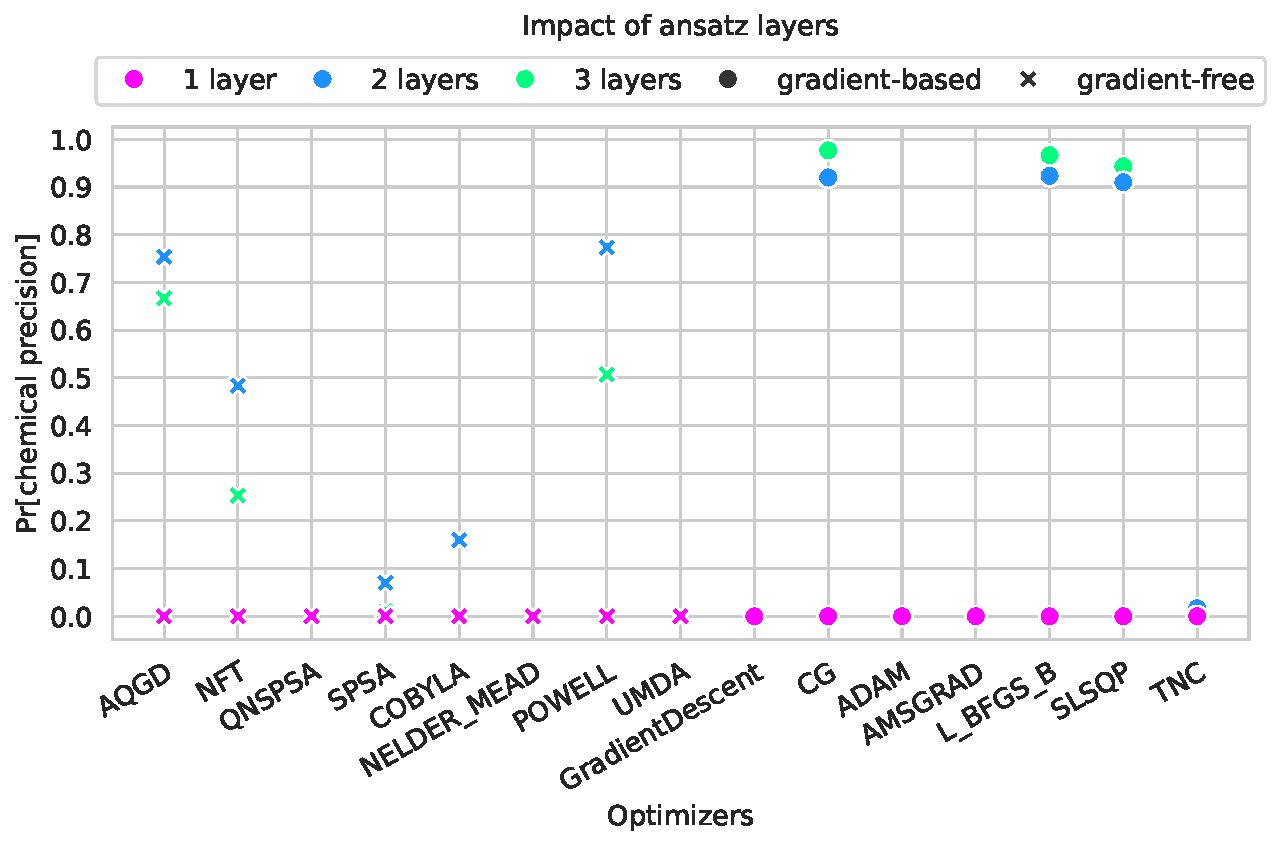
\includegraphics[width=\textwidth]{layers.pdf}
    \caption{Achieving chemical precision is unattainable using 1-layer ansatzes. Gradient-free optimizers reach better results with 2-layer ansatzes, while gradient-based optimizers perform better with 3-layer ansatzes.}
    \label{fig:ansatz-layers}
\end{figure}
One important finding we have made is the impossibility of achieving chemical precision using a 1-layer ansatz regardless of the optimizer. As depicted in Figure \ref{fig:ansatz-layers}, the probability of achieving chemical precision remains consistently zero across all optimizers for 1-layer ansatzes. Consequently, in all subsequent analyses, we excluded 1-layer ansatzes and focused exclusively on 2-layer and 3-layer ansatzes. Additionally, we observed an intriguing trend that gradient-based optimizers tend to perform better with 3-layer ansatzes, whereas gradient-free optimizers achieve better results with 2-layer ansatzes. We attribute this finding to the number of parameters that need to be optimized. We guess that gradient-free algorithms can get lost more easily in bigger spaces and gradient-based optimizers can better navigate the space thanks to gradients. However, we have not taken further steps to verify this hypothesis. 

\begin{figure}[H]
    \centering
    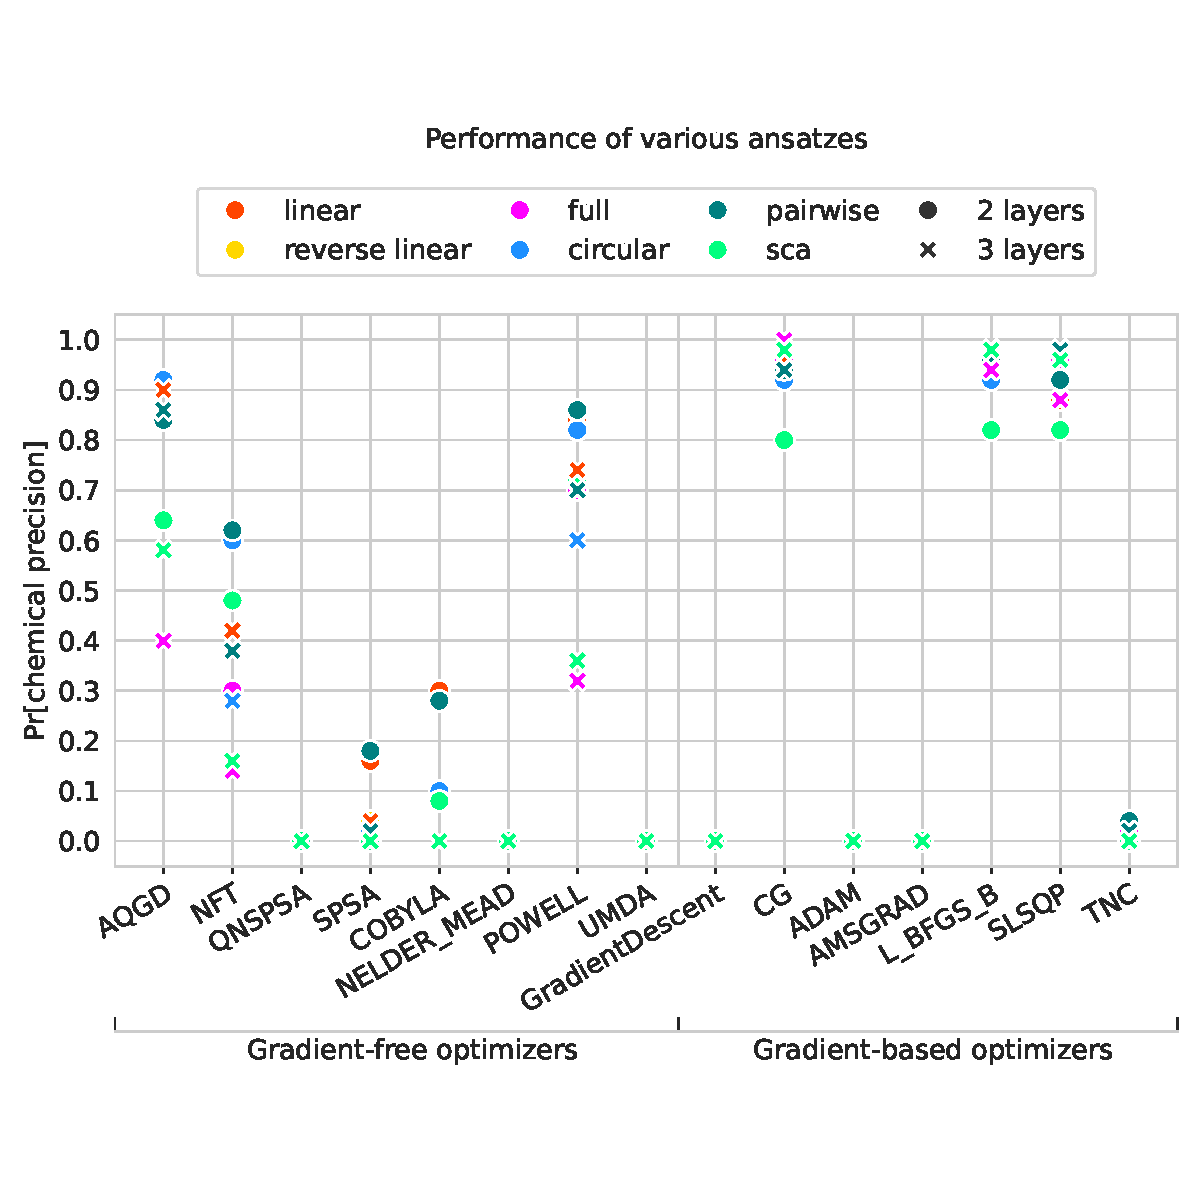
\includegraphics[width=\textwidth]{chemical.pdf}
    \caption{More detailed version of the previous figure showing also types of ansatzes with different number of layer. Gradient-based optimizers either achieve success across all tested ansatzes or fail completely. The choice of ansatz seems to have a greater impact with gradient-free optimizers.}
    \label{fig:chemical}
\end{figure}

In Figure~\ref{fig:ansatz-layers}, we were interested in ansatz layers. Figure~\ref{fig:chemical} is very similar but in addition to that, it also takes into account types of ansatzes. The figure may seem a bit unclear due to the amount of overlapping data points. In general, it is not possible to say which ansatz is the best but if we split our results into gradient-based and gradient-free optimizers we can observe some trends. When it comes to gradient-based, there are not any significant differences between ansatzes. Either an optimization algorithm works and can reach a good result with any of the tested ansatz or does not work at all. On the other hand, the performance of ansazes with gradient-free optimizers is more fragmented. The SCA and full ansatzes seem to be the worst with gradient-free optimizers. The best results are achieved with the pairwise, linear, and circular ansatzes. Surprisingly, there is a single combination of ansatz and optimizer that was able to reach a chemical precision in all 50 runs. The combination is constituted by the 3-layer full ansatz and \textit{Conjugate Gradient (CG)} optimizer.

\section{Optimizers}
The previous section indicated something about optimizers but it was more geared towards the performance of ansatzes. In this section, we will try to discuss the performance of individual optimizes in more detail by presenting the results in two distinct manners.

\begin{figure}[H]
    \centering
    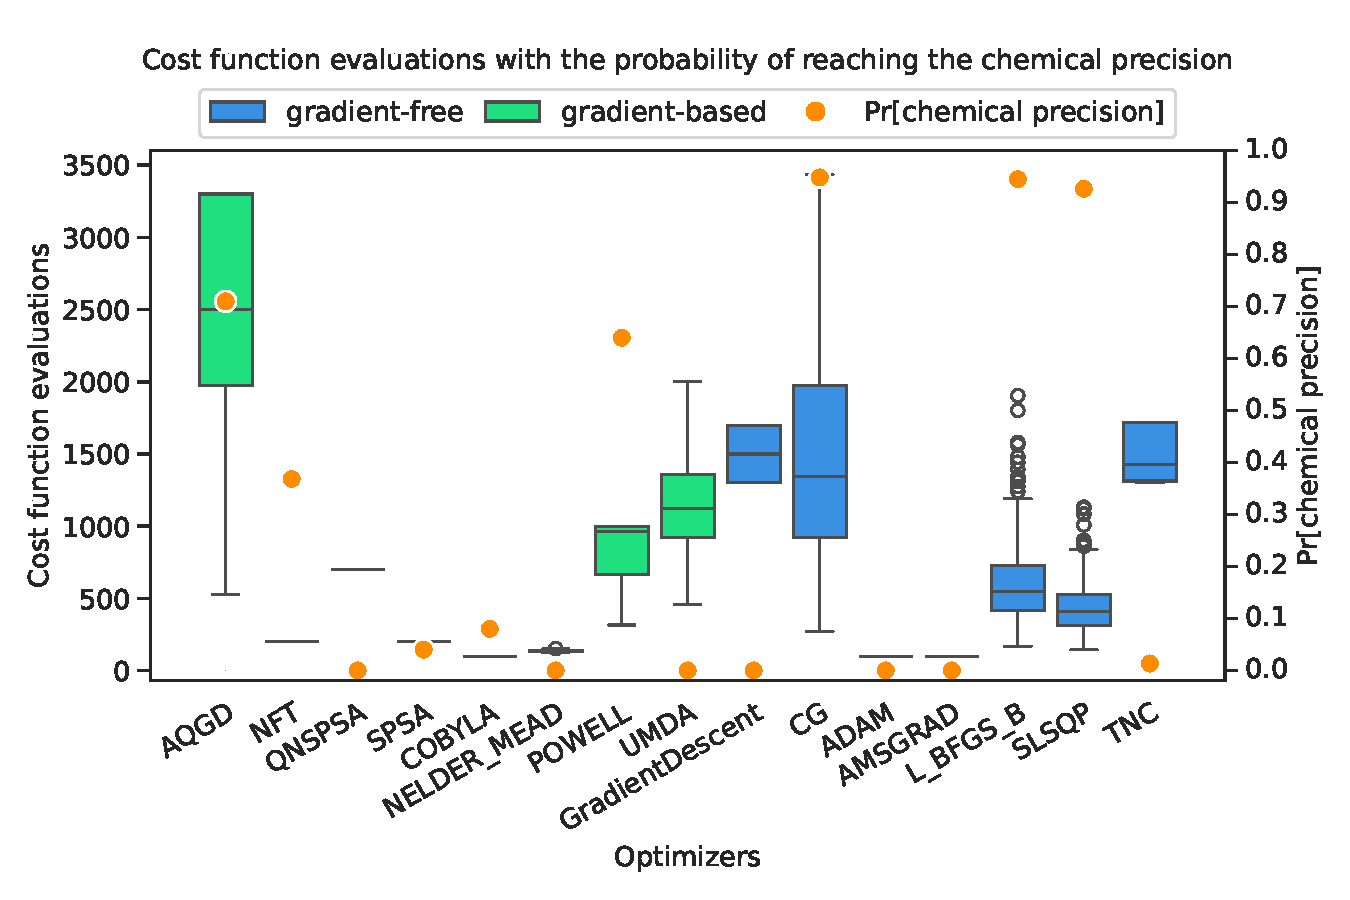
\includegraphics[width=\textwidth]{evaluations.pdf}
    \caption{Relationship between the number of cost function evaluations and the probability of achieving chemical precision for various optimizers. The performance of some optimizers appears to be constrained by a fixed cost function evaluation count. However, there are exceptions that achieved very good results despite having fewer cost function evaluations.}
    \label{fig:evaluations}
\end{figure}

Figure~\ref{fig:evaluations} depicts a visualization where the left y-axis shows the number of cost function evaluations, while the right y-axis shows the probability of reaching the chemical precision. The straight lines that we can see on \textit{NFT}, \textit{QNSPSA}, \textit{SPSA}, \textit{COBYLA}, \textit{ADAM}, and \textit{AMSGRAD} mean that these optimizers have a fixed number of cost function evaluations. It seems that a fixed number of cost function evaluations can have a limiting impact on the optimizers. Multiple optimizers that have a smaller number of cost function evaluations are not very likely to reach a chemical precision, however, \textit{L\_BFGS\_B} and \textit{SLSQP} achieved very good results despite the lower number of cost function evaluations. The \textit{Conjugate Gradient} has the best probability overall, however, it necessitates a considerable number of cost function evaluations. On the other hand, \textit{Gradient Descent} and \textit{TNC} algorithms do not work at all even though the number of cost function evaluations is not so small.

\begin{figure}[H]
    \centering
    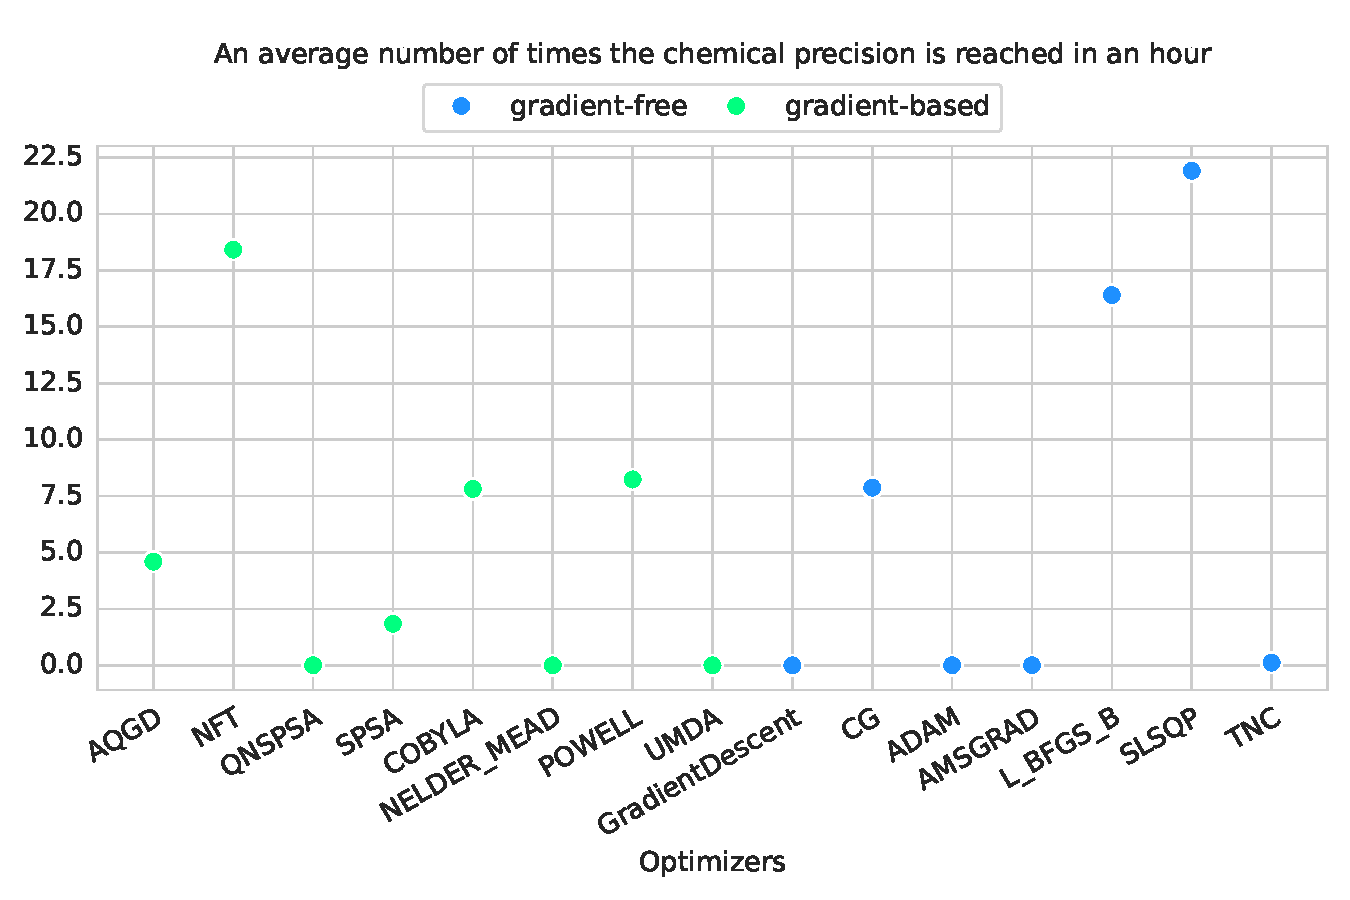
\includegraphics[width=\textwidth]{hours.pdf}
    \caption{Another point of view on the data shown in the previous figure. Such a view favors fast optimizers and they can reach solid results despite the lower probability of reaching the chemical precision.}
    \label{fig:hours}
\end{figure}

In Figure~\ref{fig:hours} we can see the average number of times the chemical precision is reached in an hour (on our hardware). This gives us a different view of the results. For instance, the \textit{NFT} optimizer does not have even 50\% probability of reaching a chemical precision, however, due to its low amount of cost function evaluations the whole execution of the algorithm is fast and therefore we can reach a chemical precision more times in an hour than with other optimizers. On the other hand, the \textit{AQGD} with a high number of cost function evaluations and with the probability of reaching the chemical precision over 70\% can yield correct results on average only nearly 5 times in an hour. This view of the data favors optimizers that are fast, they can achieve good results even though the probability of achieving chemical precision is low.

Initially, after running all the experiments, we did not consider chemical precision and we thought that gradient-free optimizers perform better due to their faster energy convergence. However, after introducing the chemical precision it turned out that the opposite is true, gradient-free optimizers have difficulties getting close enough to the ground state energy.

As a clear winner seems the \textit{SLSQP} algorithm that leads in both graphs. It has a very high probability of reaching a chemical precision, a smaller number of cost function evaluations and it was able to reach a chemical precision with all tested ansatzes without any significant difference in results. Nevertheless, the best optimizer can vary from the situation. Sometimes we strive to minimize the number of cost function evaluations since at the end of the day it can be what we pay for. Around half of the optimizers have the probability of reaching the chemical precision 0\% or close to 0\%, they were unable to tackle this problem. There may be a chance to enhance the results by increasing the number of iterations and fine-tuning the parameters of optimizers, particularly those utilizing gradients, as some of these gradient-based optimizers exhibit good performance. However, we have not taken any steps in that direction.